\section{Auswertung}
\subsection{Schallgeschwindigkeit im Acrylblock}
\label{sec:ausw_schallgeschw}

\begin{table}
    \centering
    \sisetup{table-format=2.2}
    \begin{tabular}{S S S}
        \toprule
        {$x_A/\unit{\mm} $} & {$D/\unit{\mm}$} & {$x_B/\unit{\mm}$}\\
        \midrule
        15.40   &  10.00    & 55.00         \\
        71.00   &  2.85     & 6.55          \\
        62.80   &  2.90     & 14.70         \\
        55.00   &  2.85     & 22.55         \\
        47.10   &  2.85     & 30.45         \\
        38.90   &  2.95     & 38.55         \\
        30.75   &  3.90     & 45.75         \\
        22.10   &  4.95     & 53.35         \\
        13.30   &  5.90     & 61.20         \\
        61.15   &  1.45     & 17.80         \\
        59.50   &  1.45     & 19.45         \\
        \bottomrule
    \end{tabular}
    \caption{Abmessungen des Acrylblocks}
    \label{tab:messungen}
\end{table}
Die Entfernungen der Fehlstellen vom Rand des Acrylblocks von der Seite A werden in Tabelle \ref{tab:messungen} mit $x_A$ bezeichnet.
Anhand des Lochdurchmessers $D$ wird und des Blockdurchmessers $x_\text{Block} = \qty{80.40}{\mm}$ wird der 
Abstand zum Rand des Blocks auf der B-Seite errechnet.
Diese Messungen werden in \ref{tab:schallzeit} den Ergebnissen des A-Scans gegenübergestellt.
Die Laufzeit des Schalls zur Fehlstelle und zurück wird mit $t_A$ und $t_B$ angegeben.
Zur Berechnung der Schallgeschwindigkeiten $c_A$ und $c_B$ wird von dieser Laufzeit \qty{1}{\micro\s} abgezogen,
um die Verzögerung im Wasser und in der Sonde auszugleichen. 
Dieser Wert entsteht durch vergleichen der Ergebnisse von verschiedenen verschiebungskonstanten mit dem Literaturwert der Schallgeschwindigkeit
im Acrylglas.
\begin{table}[h]
    \centering
    \sisetup{table-format = :.0}
    \begin{tabular}[pos]{S S S S S S S}
        \toprule
        {Nr.}& {$t_A/\unit{\micro\s}$} &{$t_\text{A, korr}/\unit{\micro\s}$} &
        {$t_B/\unit{\micro\s}$} & {$t_\text{B, korr}/\unit{\micro\s}$} & 
        {$c_a/\unit{\meter\per\second}$} & {$c_b/\unit{\meter\per\second}$} \\
        \midrule
        1       &  12    &  11    & 42   &  41     & 2800      & 2683     \\
        3       &  47    &  46    & 12   &  11     & 2730      & 2673     \\
        4       &  41    &  40    & 18   &  17     & 2750      & 2653     \\
        5       &  35    &  34    & 23   &  22     & 2771      & 2768     \\
        6       &  29    &  28    & 30   &  29     & 2779      & 2659     \\
        7       &  23    &  22    & 35   &  34     & 2795      & 2691     \\
        8       &  17    &  16    & 40   &  39     & 2763      & 2736     \\
        \bottomrule
    \end{tabular}
    \caption{Laufzeiten und Schallgeschwindigkeiten im Acrylblock}
    \label{tab:schallzeit}
\end{table}
Aus den Werten in Tabelle \ref{tab:schallzeit} wird der Mittelwert $\overline{c}$ und die Standardabweichung $\Delta c$ der Messungen mit folgenden Formeln berechnet:
\begin{align}
    \overline{c} &= \frac{1}{N} \sum_{k=1}^{N} c_k & \Delta c = \sqrt{ \sum_{k=1}^{N} \left(\overline{c} - c_k \right)^2 }
\end{align}
mit $N=14$ Messungen $c_k$ aus Tabelle \ref{tab:schallzeit}.
Es ergibt sich eine Schallgeschwindigkeit von $c = \qty{2730 +- 50}{\meter\per\second}$.

\subsection{Messung der Fehlstellen mit dem A-Scan}
\label{sec:ausw_fehlste}
Um die Tiefe der Fehlstellen korrekt zu bestimmen muss die Korrektur, die bei der Laufzeit für die Schallgeschwindigkeit aufgestellt wurde
mit eingerechnet werden. 
Dazu wird die Strecke $s_1 = \frac{1}{2}\qty{2730}{\meter\per\second} \cdot \qty{1e-6}{\s}= \qty{1.365}{\milli\meter}$ 
von der im Computerprogramm berechneten Strecke abgezogen.
Die abgelesene Tiefe des Blocks $s_\text{Block}$ kann so von \qty{81.5}{\mm} auf \qty{80.14}{mm} korrigiert werden was deutlich
näher am wahren Wert $x_\text{Block} = \qty{80.40}{\mm}$ liegt.
Mit den korrigierten Messwerten für die Tiefe des Blocks und die tiefen der Fehlstellen von den Seiten A und B lassen sich die
Durchmesser der Fehlstellen berechnen.
In Tabelle \ref{tab:a-scan} werden die gemessenen Tiefen $s_A$ und $s_B$ und die berechneten Durchmesser $D_s$ den 
mit der Schieblehre gemessenen Durchmessern $D$ gegenübergestellt. 
Bei der Messung für Loch Nr. 2 von Seite A konnte kein Wert erhoben werden, da das Loch 1 im Weg war.
\begin{table}[h]
    \centering
    \sisetup{table-format=2.1}
    \begin{tabular}[pos]{S[table-format = 1.0] S S S S S S}
        \toprule
        {Nr} & {$s_\text{A}/\unit{mm}$} & {$s_\text{A, korr}/\unit{mm}$} & %
        {$s_\text{B}/\unit{mm}$} & {$s_\text{B, korr}/\unit{mm}$} & %
        {$D_\text{s}/\unit{mm}$} & {$D/\unit{mm}$}\\
        \midrule
        1       &  16.5          & 15.1          & 56.5          & 55.1          & 9.9   & 10.0  \\
        2       &  {-}           & {-}           & 8.5           & 7.1           & {-}   & 2.9   \\
        3       &  64.0          & 62.6          & 16.5          & 15.1          & 2.4   & 2.9   \\
        4       &  56.5          & 55.1          & 24.0          & 22.6          & 2.4   & 2.9   \\
        5       &  48.5          & 47.1          & 32.0          & 30.6          & 2.4   & 2.9   \\
        6       &  40.0          & 38.6          & 40.0          & 38.6          & 2.9   & 3.0   \\
        7       &  31.5          & 30.1          & 47.5          & 46.1          & 3.9   & 3.9   \\
        8       &  23.0          & 21.6          & 55.0          & 53.6          & 4.9   & 5.0   \\
        9       &  14.5          & 13.1          & 62.5          & 61.1          & 5.9   & 5.9   \\
        10      &  62.5          & 61.1          & 19.0          & 17.6          & 1.4   & 1.4   \\
        11      &  61.0          & 59.6          & 21.0          & 19.6          & 0.9   & 1.4   \\
        \bottomrule
    \end{tabular}
    \caption{Messung der Fehlstellen mithilfe des A-Scans}
    \label{tab:a-scan}
\end{table}


\subsection{Auflösungsvermögen}
\label{sec:ausw_aufl}
Bei der Untersuchung der doppelten Fehlstelle ergibt sich, in der Messung mit der \qty{2}{\mega\hertz} Sonde, 
ein  Bild bei dem zwei verschiedene Peaks zu erkennen sind (vgl. Abbildung \ref{fig:aufloesung_b}).
Bei der Messung mit \qty{1}{\mega\hertz} ist das nicht möglich.

\begin{figure}[h]%
    \begin{subfigure}{0.48\textwidth}%
        \centering%
        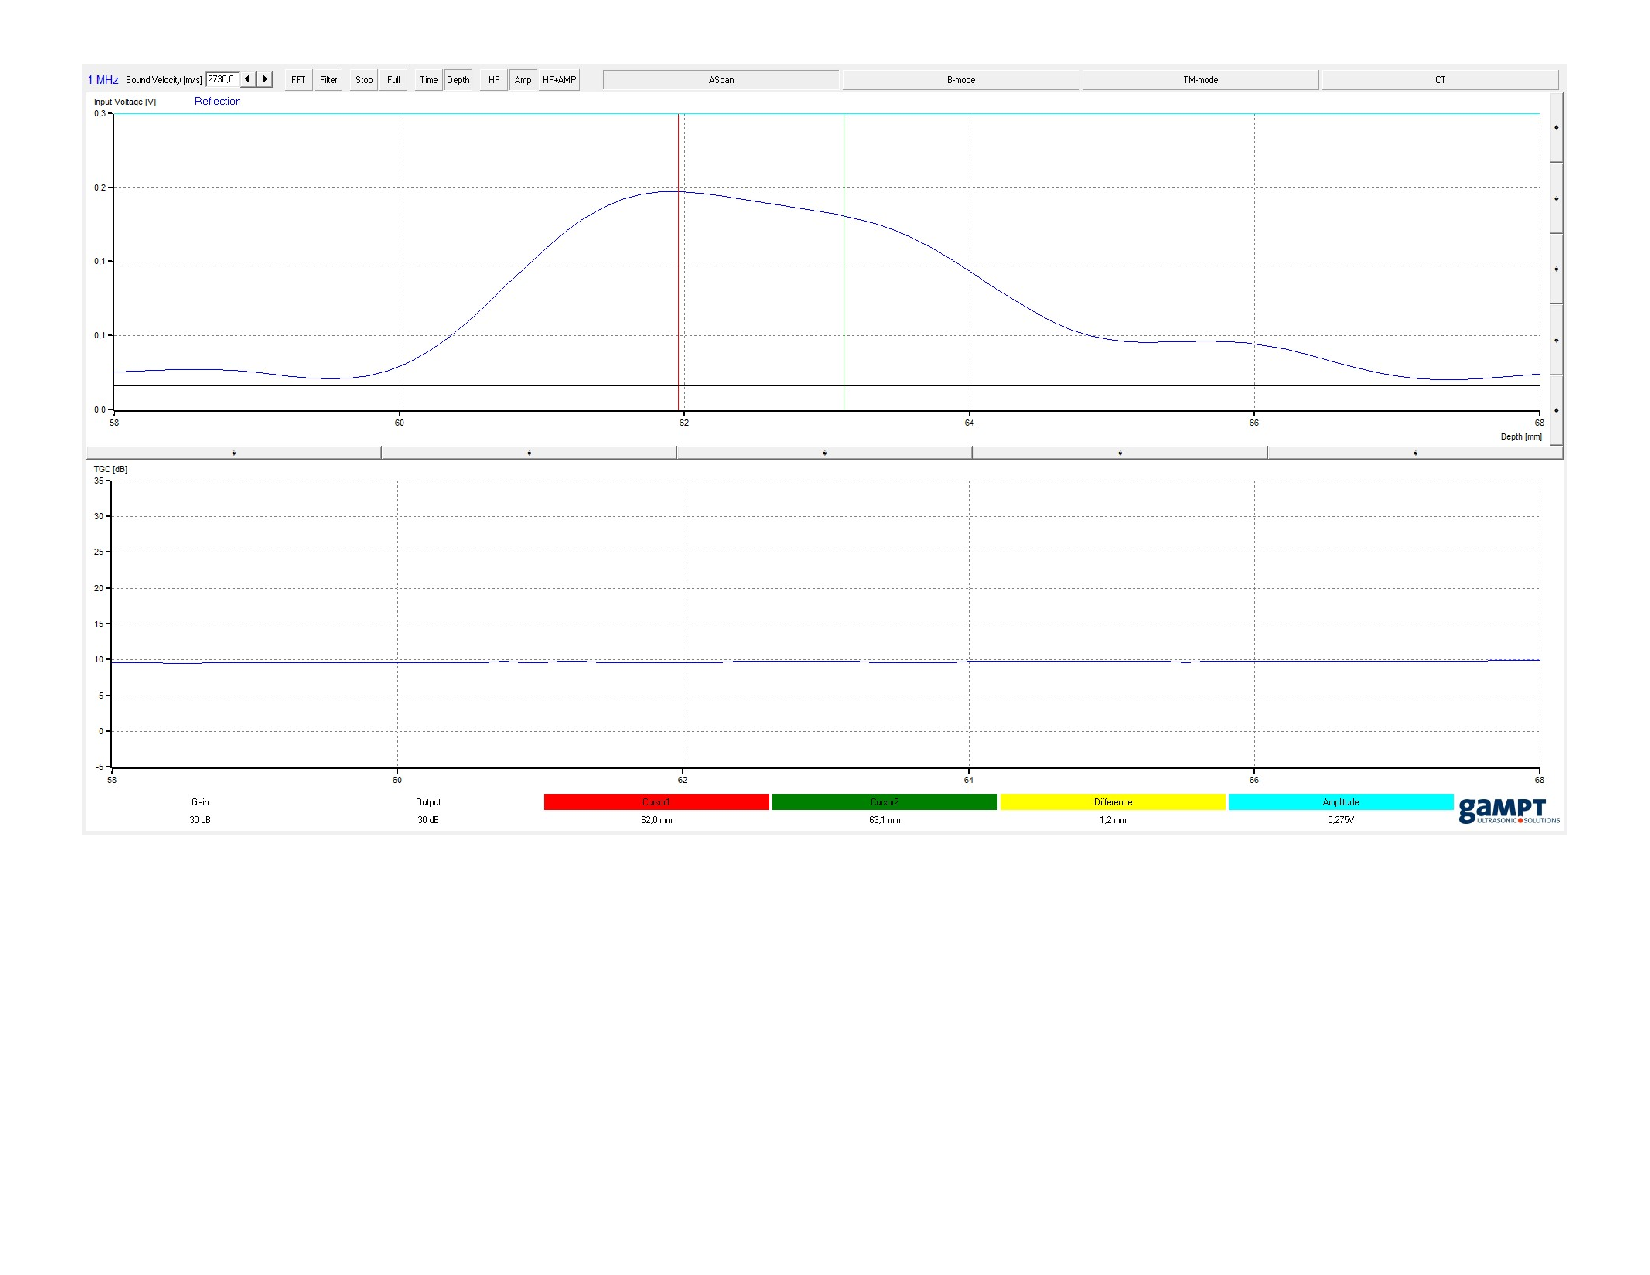
\includegraphics[width=\textwidth]{Messdaten/aufloesung 1mhz zoom.pdf}%
        \caption{\qty{1}{\mega\hertz}.}%
        \label{fig:aufloesung_a}%
    \end{subfigure}%
    \hfill%
    \begin{subfigure}{0.48\textwidth}%
        \centering%
        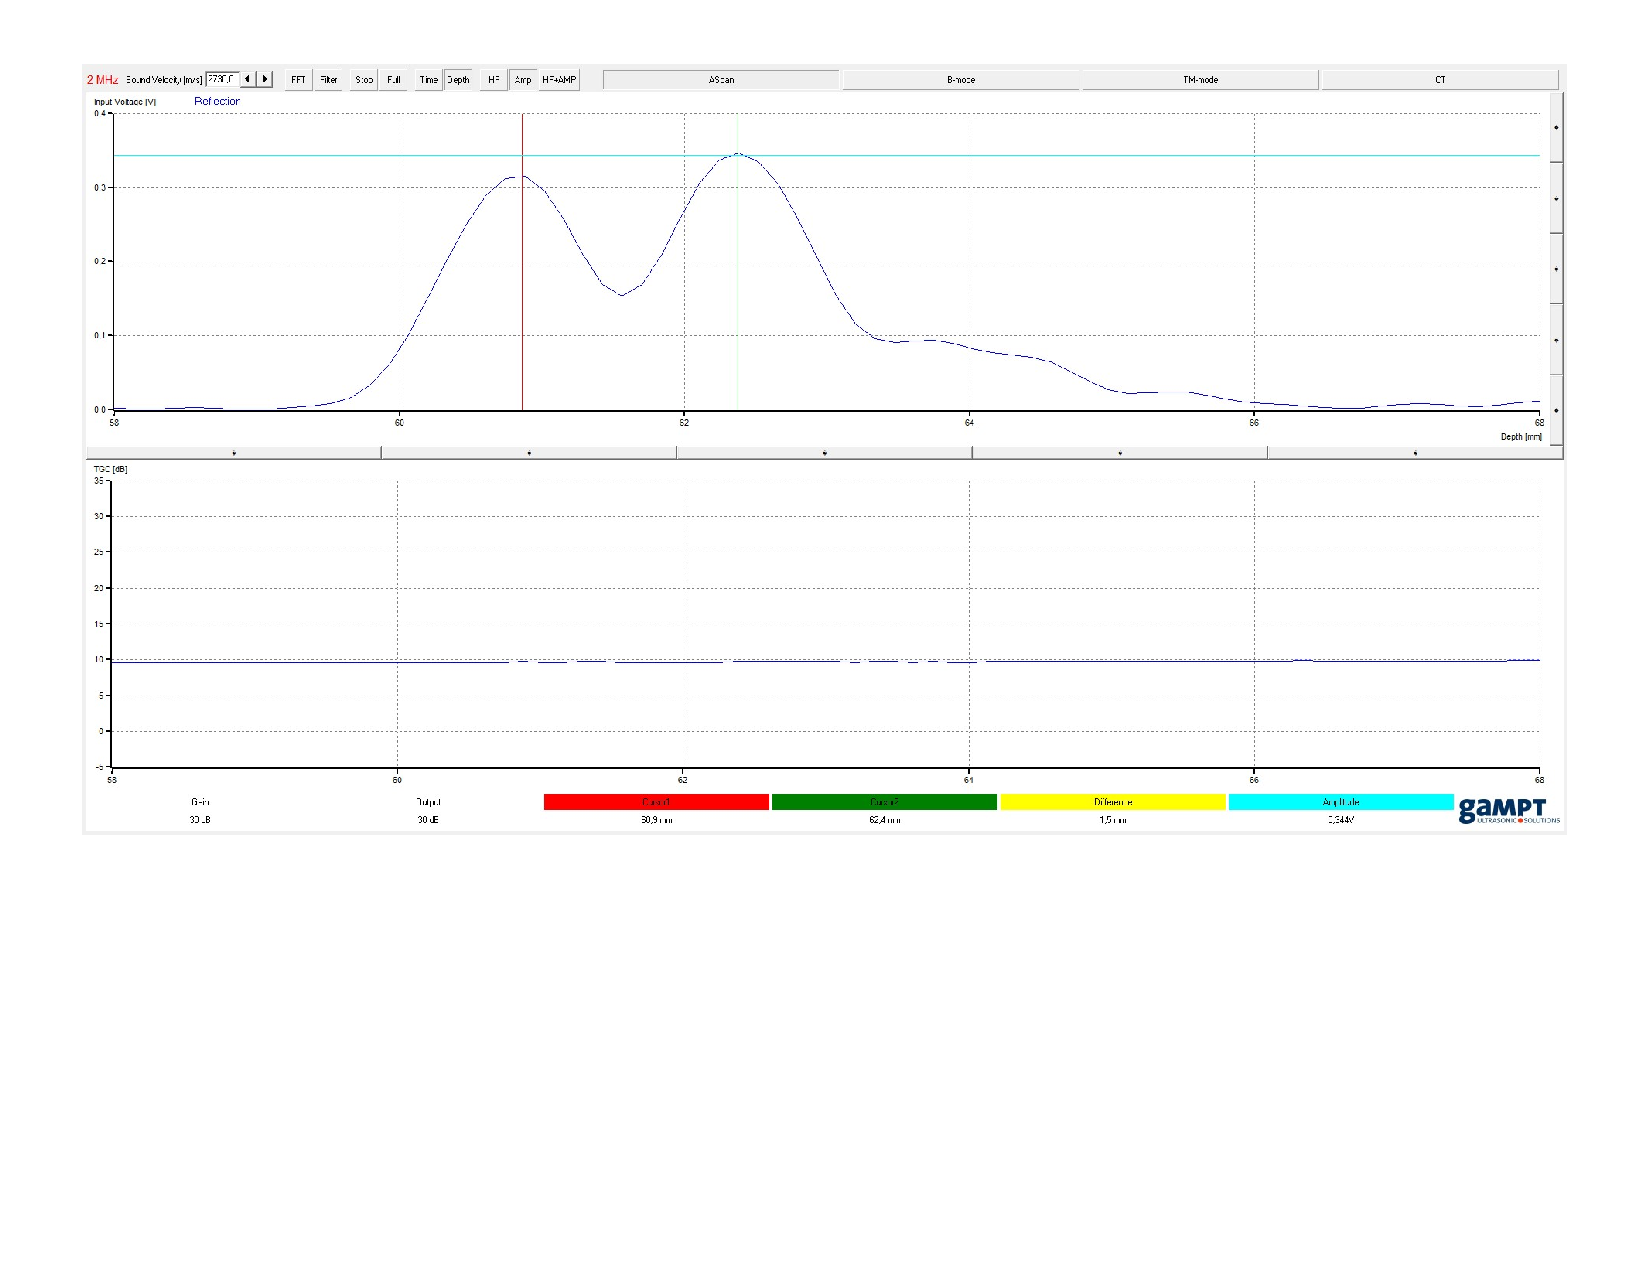
\includegraphics[width=\textwidth]{Messdaten/aufloesung 2mhz zoom.pdf}%
        \caption{\qty{2}{\mega\hertz}.}%
        \label{fig:aufloesung_b}%
    \end{subfigure}%
    \caption{Die Fehlstellen bei unterschiedlichen Frequenzen.}%
    \label{fig:aufloesung}%
\end{figure}%

\subsection{B-Scan am Acrylblock}
\label{sec:ausw_B}
\begin{figure}[h]
    \begin{subfigure}{0.48\textwidth}
        \centering
        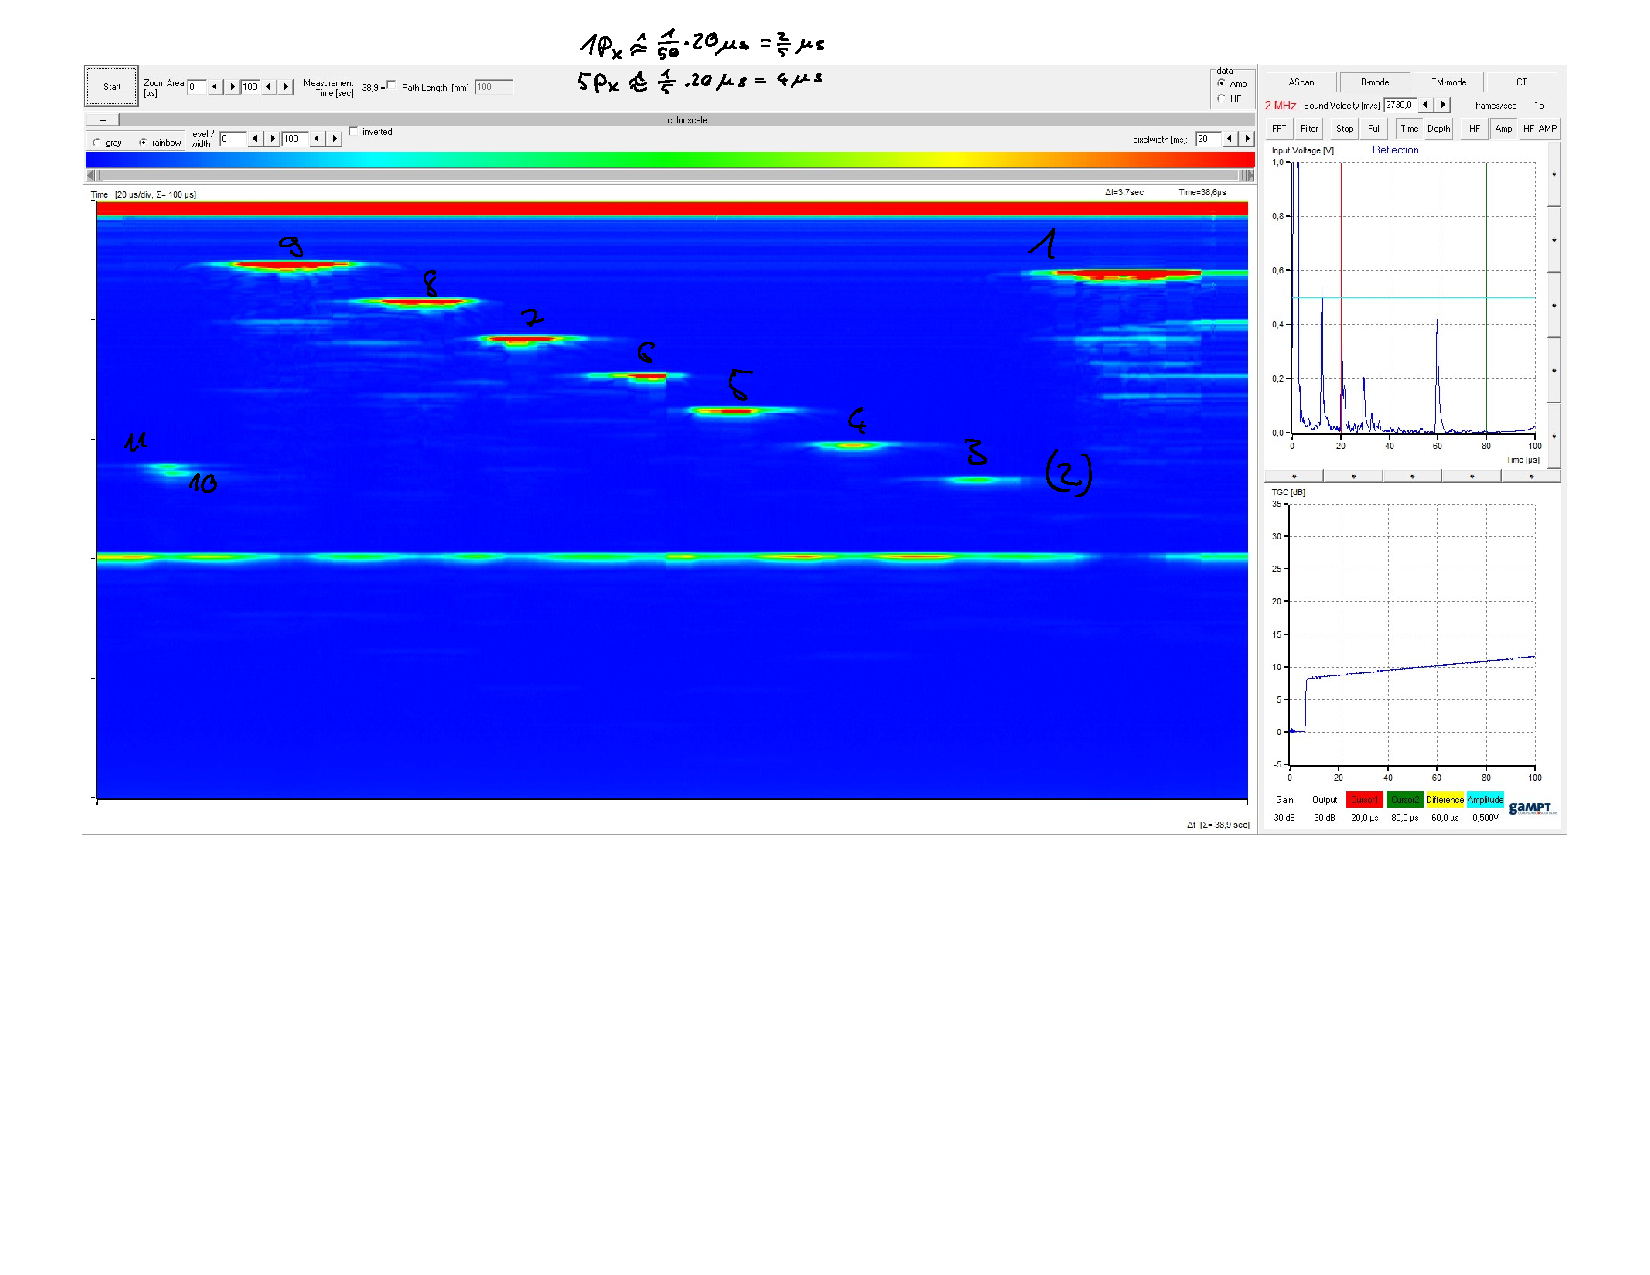
\includegraphics[width=\textwidth]{Abbildungen/b scan acryl 1-Copy.pdf}
        \caption{Seite A, absteigende Nummerierung.}
    \end{subfigure}
    \hfill
    \begin{subfigure}{0.48\textwidth}
        \centering
        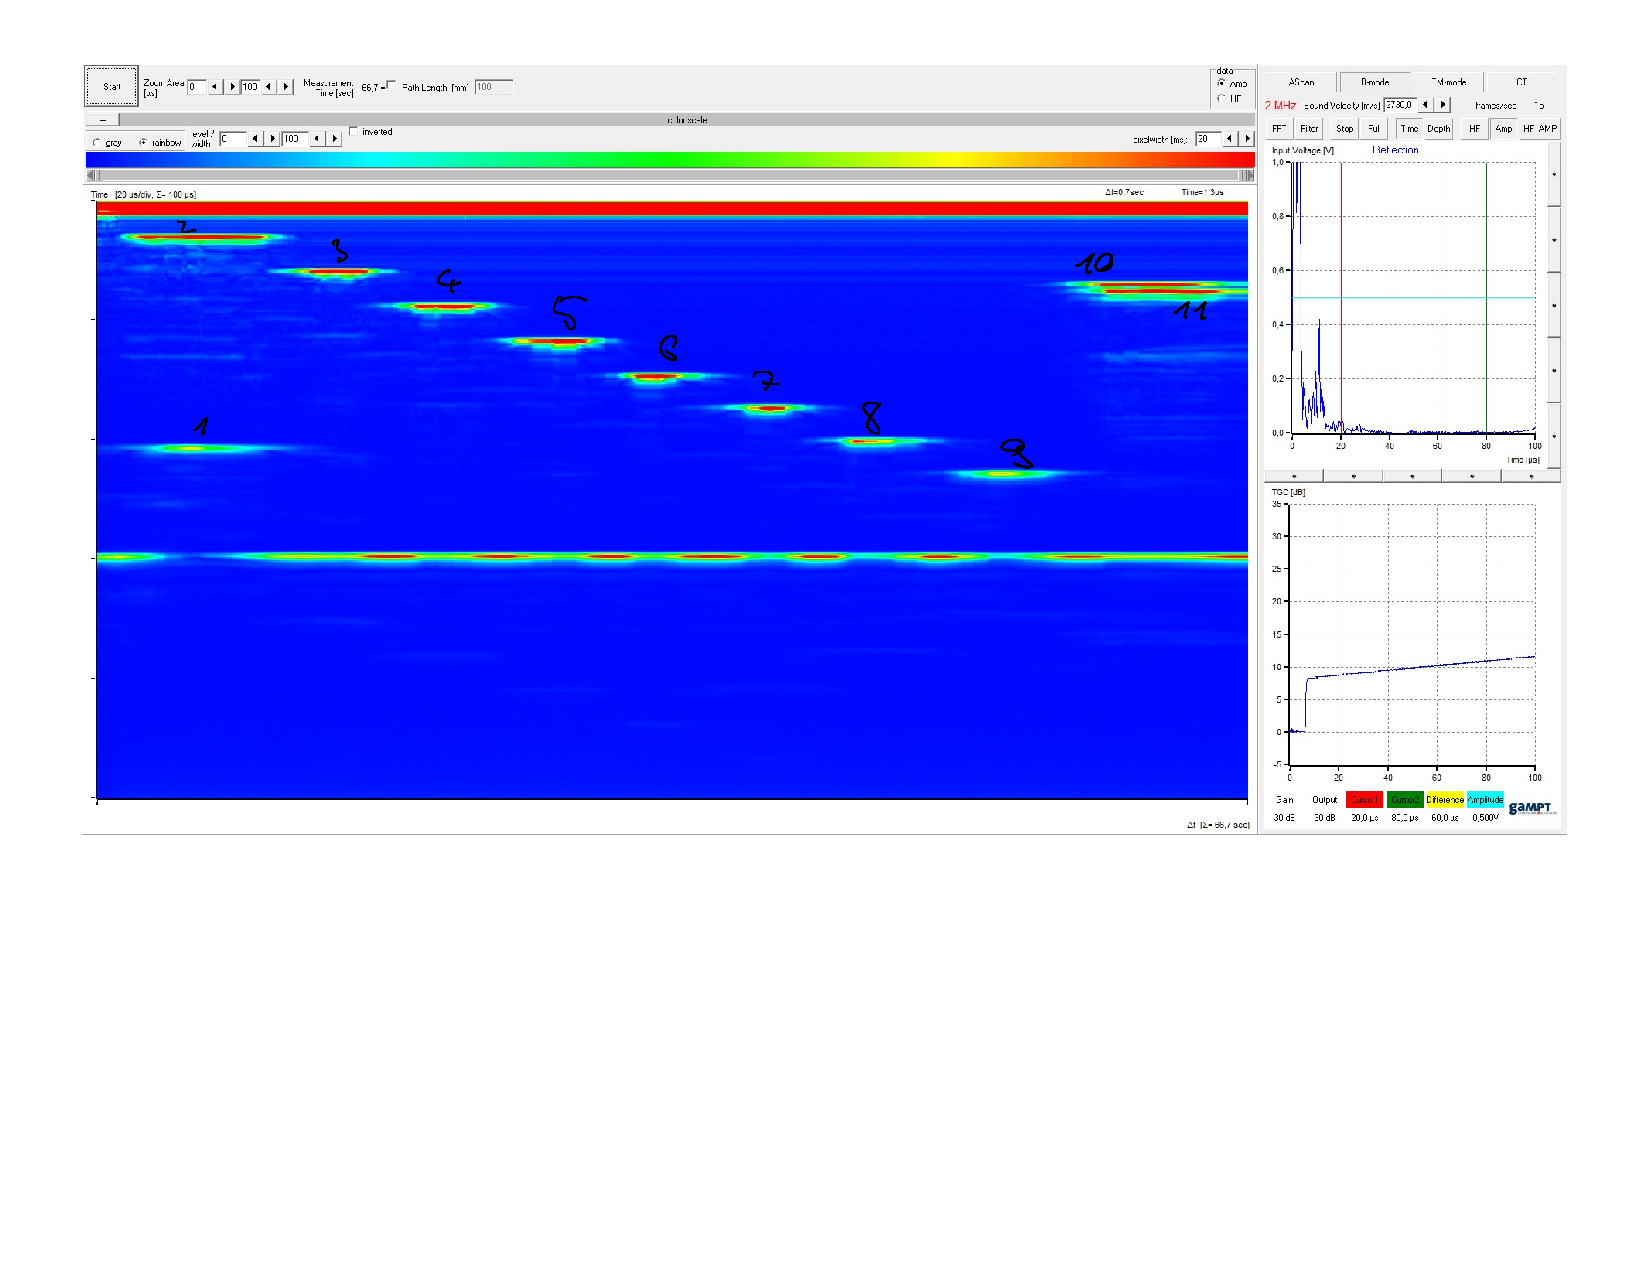
\includegraphics[width=\textwidth]{Abbildungen/b scan acryl 1 rueckseite-Copy.pdf}
        \caption{Seite B, aufsteigende Nummerierung.}
    \end{subfigure}
    \caption{Ergebnisse des B-Scans des Acrylblocks}
    \label{fig:b-scan}
\end{figure}

\begin{table}[h]
    \centering
    \sisetup{table-format=:.1}
    \begin{tabular}{S[table-format=:.0] S S S S S S}
        \toprule
        {Nr}& {$t_A/\unit{\micro\second}$} & {$t_B/\unit{\micro\second}$} &
        {$x_A/\unit{\mm}$} & {$x_B/\unit{\mm}$} & {$D_\text{sb}/\unit{\mm}$}& {$D/\unit{\mm}$}\\
        \midrule
        1       & 12.4  & 41.6  & 15.6  & 55.4  & 9.8  & 10.0 \\
        2       & {-}   & 6.2   & {-}   & 7.1   & {-}  & 2.9  \\
        3       & 46.6  & 11.9  & 62.2  & 14.9  & 3.7  & 2.9  \\
        4       & 40.8  & 18.1  & 54.3  & 23.3  & 3.1  & 2.9  \\
        5       & 35.1  & 24.0  & 46.5  & 31.4  & 2.9  & 2.9  \\
        6       & 29.3  & 29.9  & 38.6  & 39.4  & 2.7  & 3.0  \\
        7       & 23.1  & 35.2  & 30.2  & 46.7  & 4.0  & 3.9  \\
        8       & 16.9  & 40.9  & 21.7  & 54.5  & 4.6  & 5.0  \\
        9       & 10.8  & 46.4  & 13.4  & 62.0  & 5.5  & 5.9  \\
        10      & 45.6  & 14.7  & 60.9  & 18.7  & 1.2  & 1.4  \\
        11      & 44.4  & 15.8  & 59.2  & 20.2  & 1.4  & 1.4  \\
        \bottomrule
    \end{tabular}
    \caption{Ergebnisse der Messungen mit dem B-Scan.}
    \label{tab:b-scan}
\end{table}

Bei dem B-scan werden die Messungen analog zu Abschnitt \ref{sec:ausw_fehlste} ausgewertet.
Um die Positionen der Peaks zu bestimmen wird das online tool \enquote*{WebPlotDigitizer} \cite{webplot} verwendet.
Die Laufzeiten des Schalls werden um $t_1 = \qty{1}{\micro\s}$ korrigiert, dh. die Tiefen werden mit
$s = \frac{1}{2} c \cdot (t_\text{Laufzeit} - t_1)$
berechnet.
Für die Tiefe des Blocks ergibt sich bei einer Laufzeit von $t_\text{Block}= \qty{60.2}{\micro\s}$ eine Tiefe 
$s_\text{Block}= \qty{80.8}{\mm}$.
   
\subsection{Untersuchung eines Brustmodells mit einem B-Scan}%
\label{sec:ausw_brust}
\begin{figure}%
    \begin{subfigure}{0.48\textwidth}%
        \centering%
        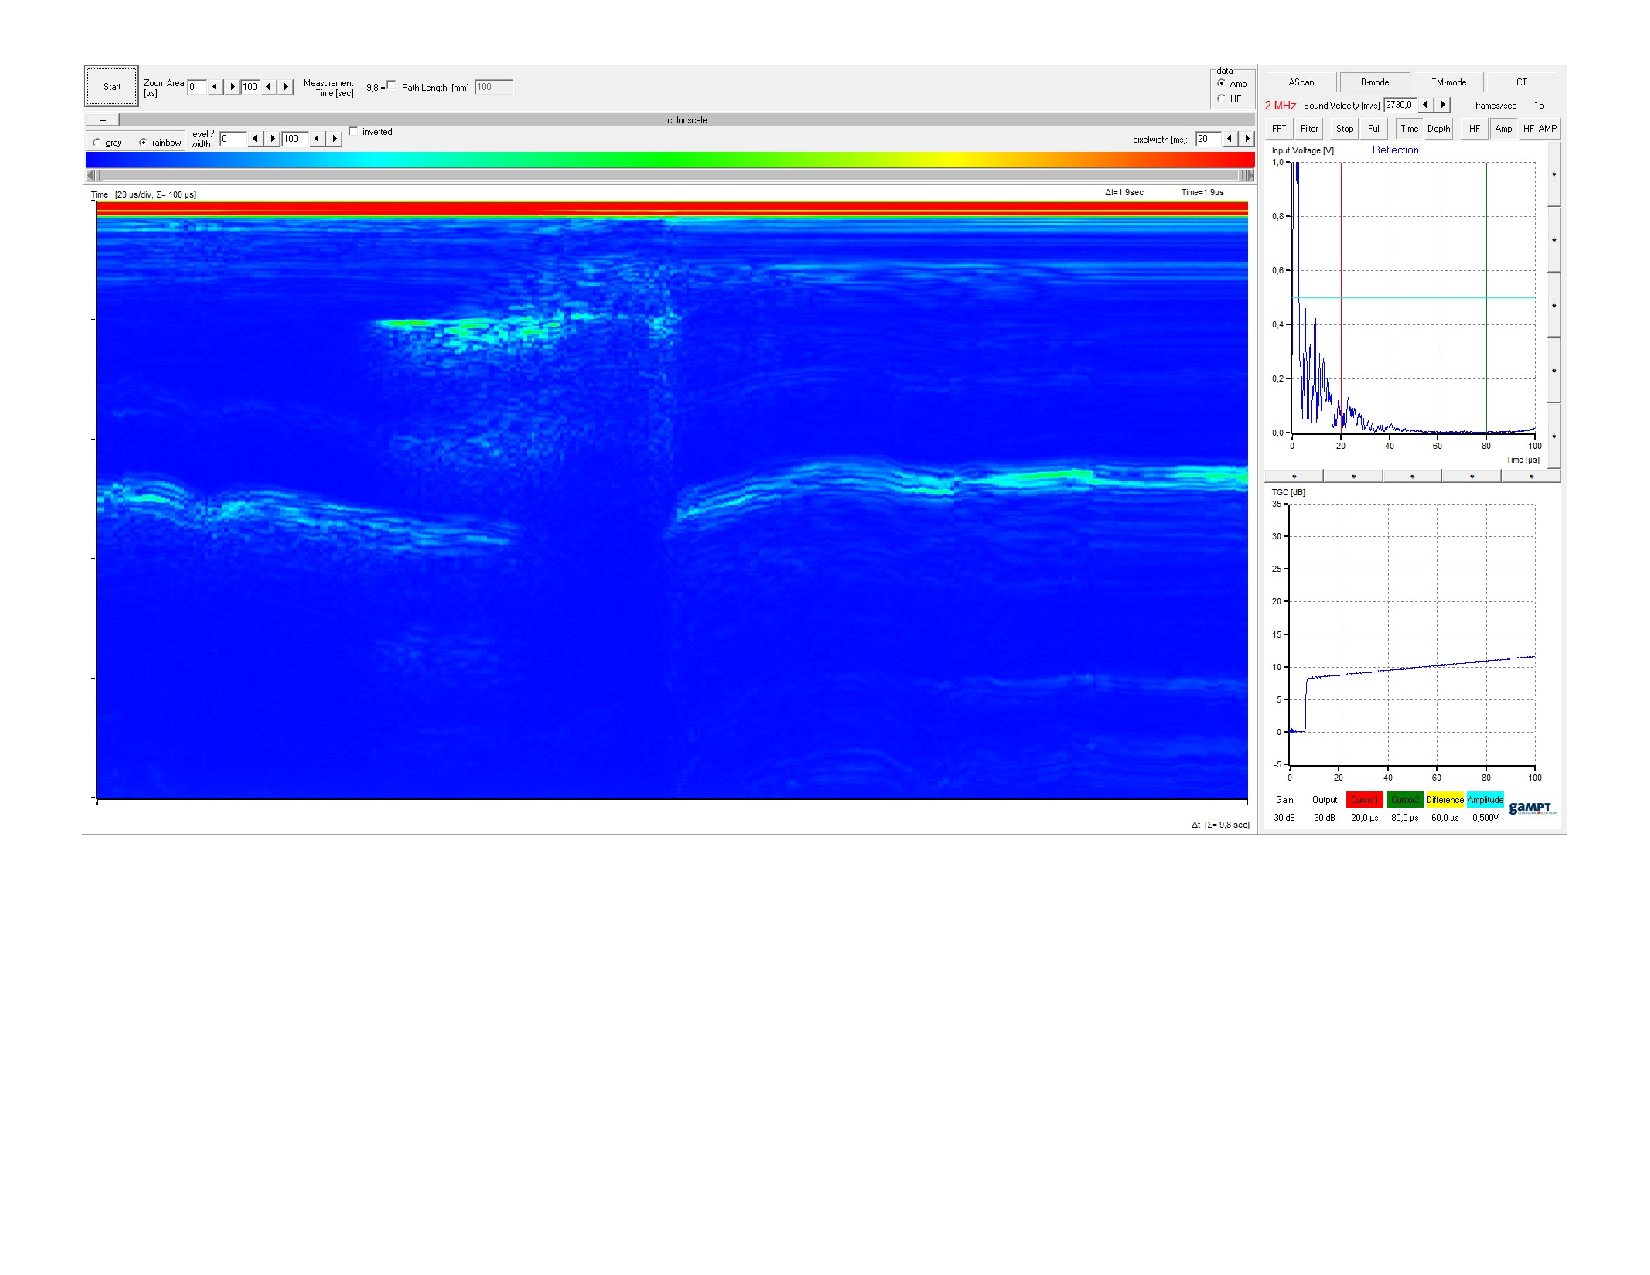
\includegraphics[width=\textwidth]{Messdaten/Tumor 1D.pdf}%
        \caption{Tumor 1.}%
        \label{fig:tumor_1}%
    \end{subfigure}%
    \begin{subfigure}{0.48\textwidth}%
        \centering%
        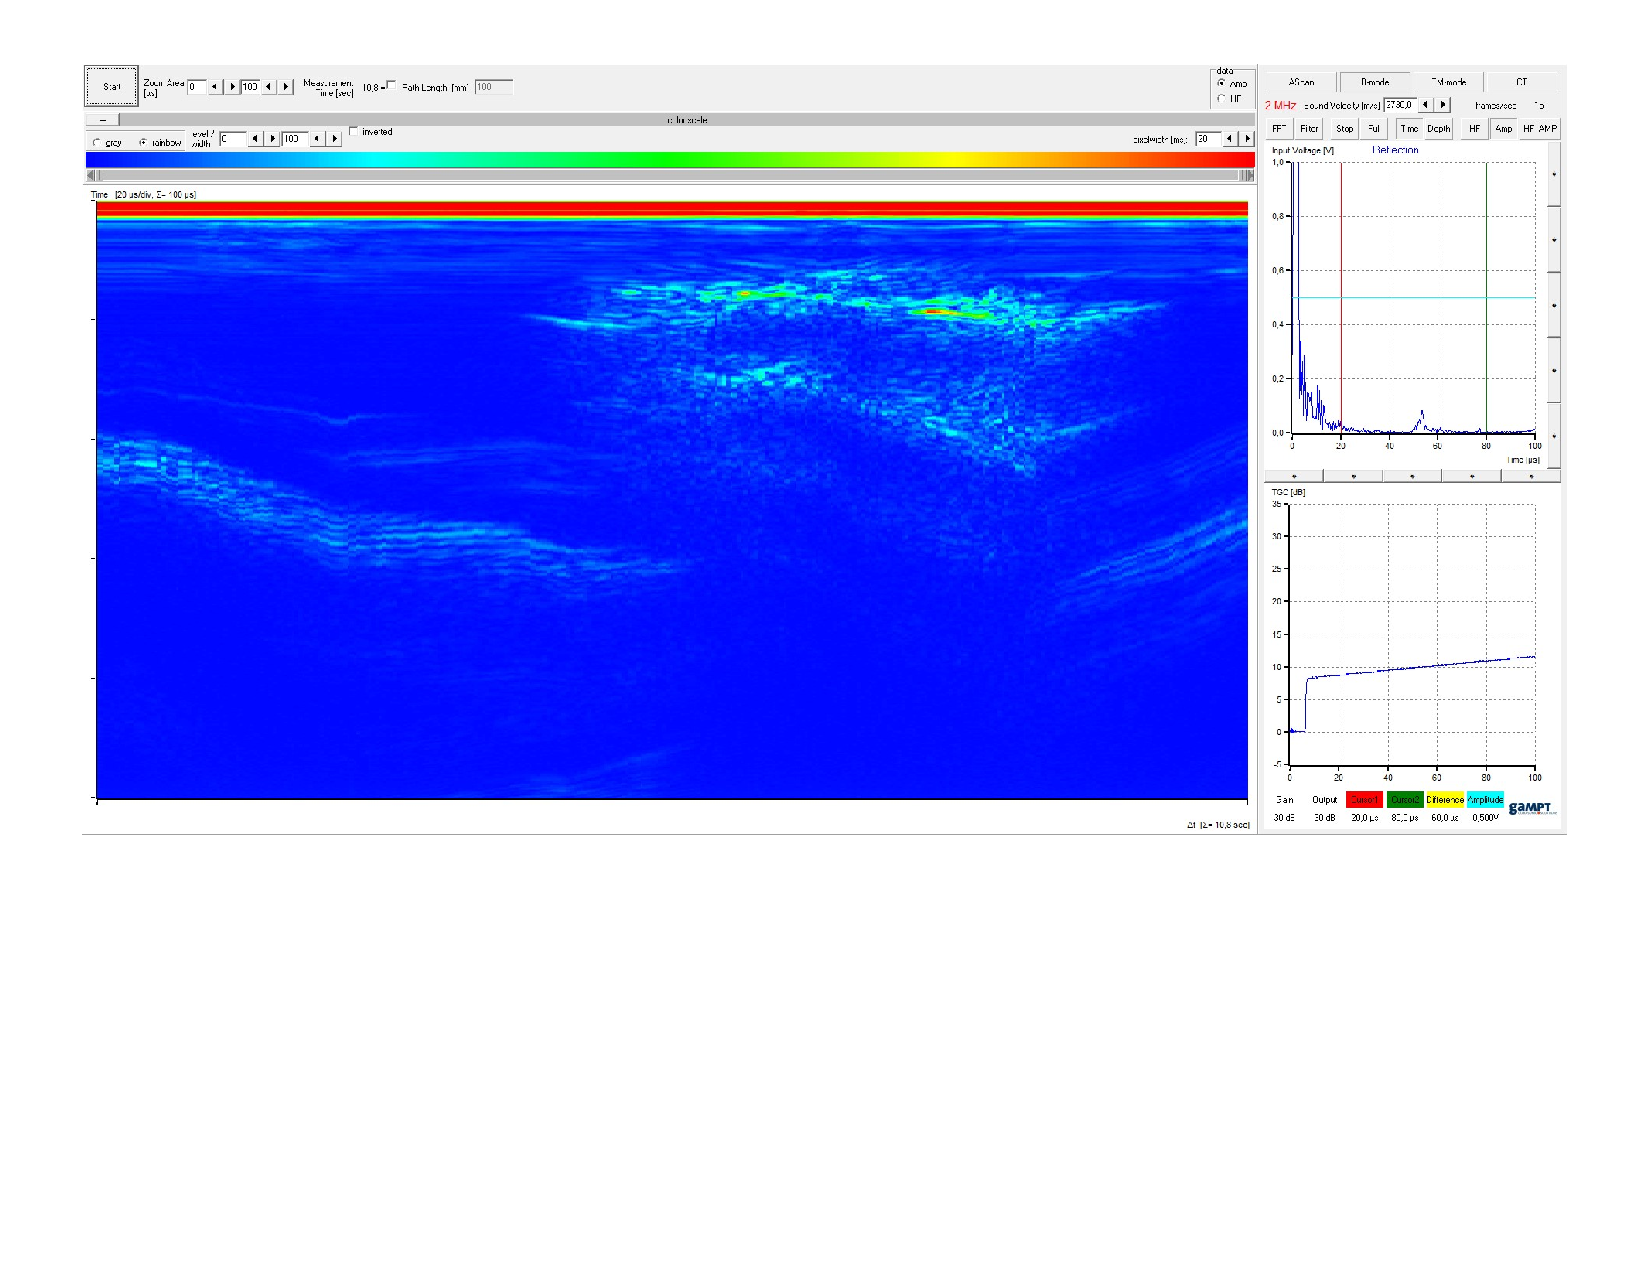
\includegraphics[width=\textwidth]{Messdaten/Tumor 2B.pdf}%
        \caption{Tumor 2.}%
        \label{fig:tumor_2}%
    \end{subfigure}%
    \caption{Tumore im Brustmodell auf dem B-Scan.}%
    \label{fig:tumore}
\end{figure}%

In den beiden Scans des Brustmodells sind zwei unterschiedliche Tumore zu erkennen.
In Abbildung \ref{fig:tumore} werden sie gegenübergestellt.
Tumor 1 sorgt in der Messung für einen kleineren Ausschlag und ist demnach aus einem dem restlichen Brustmodell ähnlicheren Material.
Der zweite Tumor ist näher an der Haut des Brustmodells als der Erste.